\section{Theoretical Analysis}
\label{sec:analysis}

\par In this section, the circuit shown in Figure~\ref{fig:Cir} is analysed
theoretically, to determine all mesh currents and nodes voltages.
In Figure~\ref{fig:Cir_teo}, conventions that will be used doing mesh and nodes analysis are shown.

\begin{figure}[H] \centering
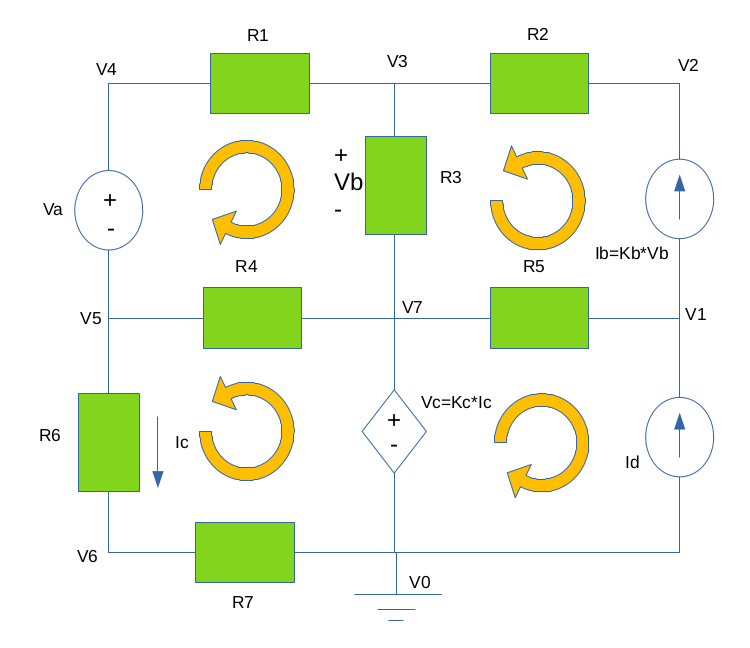
\includegraphics[width=0.8\linewidth]{Esquema_teor.png}
\caption{Circuit with nodes and currents convention}
\label{fig:Cir_teo}
\end{figure}

\par Also, the resistance, constants of the dependent sources and current values that were given by the \emph{Python} program are shown in the following table.
\vspace{5mm}
\begin{table}[H]
\centering
\begin{tabularx}{0.8\textwidth} {
  | >{\raggedright\arraybackslash}X
  | >{\raggedleft\arraybackslash}X | }
 \hline
R1 & 1.006765e+03 Ohm \\ \hline
R2 & 2.033032e+03 Ohm \\ \hline
R3 & 3.033913e+03 Ohm \\ \hline
R4 & 4.003128e+03 Ohm \\ \hline
R5 & 3.131011e+03 Ohm \\ \hline
R6 & 2.093899e+03 Ohm \\ \hline
R7 & 1.017744e+03 Ohm \\ \hline
Vs & 5.223200e+00 V \\ \hline
C & 1.035361e-06 F \\ \hline
Kb & 7.272764e-03 S \\ \hline
Kd & 8.170065e+03 Ohm \\ \hline

\end{tabularx}
\end{table}

\subsection{Mesh analysis}
\label{ssec:Mesh analysis}

\par By inspection, the circuit has four meshes. In each one, the current flows like in Figure~\ref{fig:Cir_teo}. Since there are four variables, $I_1$, $I_2$, $I_3$ and $I_4$, we'll need four linearly independent equations. To get them we'll apply KVL to mesh '1' and mesh '3' since they don't have current sources that hinder the job. the two equations will be

\begin{equation}
  Va = R1 \cdot I_1+R3(I_1 + I_2) + R4(I_1 + I_3)
  \label{eq:KVL1}
\end{equation}

\begin{equation}
  Vc = R4(I_3 + I_1) + R6 \cdot I_3 + R7 \cdot I_3
  \label{eq:KVL3}
\end{equation}

\par We can see now that in equation~\ref{eq:KVL3}, we added a new variable, $Vc$, so we'll need to find another equation. Since we know by inspection that $Ic=I_3$, we can easily get,

\begin{equation}
  Vc = Kc \cdot I_3
  \label{eq:Vc}
\end{equation}

\par Now we still need two other equations. We find one by analysing the dependent current source, the voltage drop in $R3$ and by detecting that $I_2=Ib$,

 \begin{equation}
  \frac{I_b}{Kb} = Vb = (I_1 + I_2)R3 \cdot \Rightarrow \frac{I_2}{Kb} = (I_1 + I_2)R3.
  \label{eq:Vb}
\end{equation}

\par Again, by inspection, we get $I_4 = -Id$ which finalises our equations.
To solve these equations, we put them in matrix form and then use octave to solve the matrix equation in a much easier way.

$$
\begin{bmatrix}
R1+R3+R4 & R3 & R4 & 0 \\
R4 & 0 & R4+R6+R7-Kc & 0 \\
R3Kb & R3Kb-1 & 0 & 0 \\
0 & 0 & 0 & 1 
\end{bmatrix}
\begin{bmatrix}
I1 \\
I2 \\
I3 \\
I4 
\end{bmatrix}
=
\begin{bmatrix}
Va \\
0 \\
0 \\
-Id
\end{bmatrix}
$$

\par The theoretical values are shown in the table below.
\vspace{5mm}
\begin{table}[H]
\centering
\begin{tabularx}{0.8\textwidth} {
  | >{\raggedright\arraybackslash}X
  | >{\raggedleft\arraybackslash}X | }
 \hline
I1 & 2.604926e-01 mA \\ \hline
I2 & -2.728588e-01 mA \\ \hline
I3 & 9.881466e-01 mA \\ \hline
I4 & -1.035361e+00 mA \\ \hline

\end{tabularx}
\end{table}
\vspace{5mm}

\subsection{Node analysis}
\label{ssec:Node analysis}

\par For the node analysis, we number the nodes as in Figure~\ref{fig:Cir_teo}, as said. For this method we'll work with conductance instead of resistance, because it makes it easier to work with. We now have eight variables, so we'll have to find eight equations. Since we defined ground in node zero, we get the first equation, which is $V_0=0$. The next four equations, we get from doing KCL in nodes 1, 2, 3 and 6 since they don't have voltage sources. The equations are the following\\
\vspace{5mm}
\par Node 1:

 \begin{equation}
  -Id + Ib - G5(V_7-V_1) = 0.
  \label{eq:N1}
\end{equation}

Node 2:

 \begin{equation}
  -Ib + G2(V_2-V_3) = 0.
  \label{eq:N2}
\end{equation}

Node 3:

 \begin{equation}
  -G2(V_2-V_3)-G1(V_4-V_3)-G3(V_3-V_7) = 0.
  \label{eq:N3}
\end{equation}

Node 6:

 \begin{equation}
  G7(V_6-V_0)-G6(V_5-V_6) = 0.
  \label{eq:N6}
\end{equation}

\par From these equations, we can see that we added a new unknown variable, $Ib$. For that reason, we need to add another equation - we'll use the current source and the voltage drop in $R3$. Knowing that, we get

 \begin{equation}
  I_b = Kb \cdot Vb = Kb(V_3-V_7) \Rightarrow Ib = Kb(V_3-V_7).
  \label{eq:Ib}
\end{equation}

\par We still need three equations. We'll get one from de voltage drop in $Va$, and another from the voltage drop in the dependent voltage source. These two equations are,

  \begin{equation}
  V_4-V_5 = Va
  \label{eq:Va}
\end{equation}

and

 \begin{equation}
  V_7-V_0 = Kc \cdot Ic = Kc\cdot G6(V_5-V_6) \Rightarrow V_7-V_0 = Kc\cdot G6(V_5-V_6).
  \label{eq:Vc}
\end{equation}

\par The final equation will be from the the node seven, but since we don't easily know the current that flows through the dependent current source, we first need to find a equation for this current. For that, we'll analyse node 0, which allows us to get the equation

 \begin{equation}
  I = G7(V_6-V_0) - Id
  \label{eq:corrente}
\end{equation}

\noindent where $I$ is the current we are trying to find. Now, doing the node analysis for node 7, we get the equation

 \begin{equation}
  G5(V_7-V_1)+G4(V_7-V_5)-G3(V_3-V_7)-G7(V_6-V_0)+Id = 0.
  \label{eq:N3}
\end{equation}

\par We finaly have a sistem of linearly independent equations that we can solve, using the matrix form in octave.

$$
\begin{bmatrix}
0 & G5 & 0 & Kb & 0 & 0 & 0 & -G5-Kb \\
0 & 0 & G2 & -Kb-G2 & 0 & 0 & 0 & Kb \\
0 & 0 & -G2 & G2+G1+G3 & -G1 & 0 & 0 & -G3 \\
-G7 & 0 & 0 & 0 & 0 & -G6 & G7+G6 & 0 \\
G7 & -G5 & 0 & -G3 & 0 & -G4 & -G7 & G5+G4+G3 \\
0 & 0 & 0 & 0 & 1 & -1 & 0 & 0 \\
-1 & 0 & 0 & 0 & 0 & -KcG6 & KcG6 & 1 \\
1 & 0 & 0 & 0 & 0 & 0 & 0 & 0 \\
\end{bmatrix}
\begin{bmatrix}
V_0 \\
V_1 \\
V_2 \\
V_3 \\
V_4 \\
V_5 \\
V_6 \\
V_7  
\end{bmatrix}
=
\begin{bmatrix}
Id \\
0 \\
0 \\
0 \\
-Id \\
Va \\
0 \\
0  
\end{bmatrix}
$$

The theoretical values are shown in the table below.
\vspace{5mm}
\begin{table}[H]
\centering
\begin{tabularx}{0.8\textwidth} {
  | >{\raggedright\arraybackslash}X
  | >{\raggedleft\arraybackslash}X | }
 \hline
V0 & -0.000000e+00 V \\ \hline
V1 & 1.216927e+01 V \\ \hline
V2 & 7.480974e+00 V \\ \hline
V3 & 8.035705e+00 V \\ \hline
V4 & 8.297960e+00 V \\ \hline
V5 & 3.074760e+00 V \\ \hline
V6 & 1.005680e+00 V \\ \hline
V7 & 8.073223e+00 V \\ \hline

\end{tabularx}
\end{table}

\subsection{Error analysis}
\label{ssec:Error analysis}
\par As \emph{Octave}'s output (for the mesh analyses) is just the value of the circulation current in each mesh, we're going to compute the current value in each resistor, for the sake of comparison with \emph{Ngspice}'s simulation results. We'll also compute the error associated to each current value output by \emph{Ngspice}.
\vspace{5mm}

\begin{table}[H]
\centering
\begin{tabularx}{0.8\textwidth} {
  | >{\raggedright\arraybackslash}X
  | >{\centering\arraybackslash}X
  | >{\centering\arraybackslash}X
  | >{\raggedleft\arraybackslash}X | }
 \hline
 Resistor & Expression & Value [A] & Error(\%)\\
 \hline
 r1 & $I1$ & $2.604926e-4$ & $0$ \\
 \hline
 r2 & $I2$ & $-2.728588e-4$ & $7.329798416e-5$ \\
 \hline
 r3 & $I1+I2$ & $-1.23662e-5$ & $0$ \\
 \hline
 r4 & $I1+I3$ & $1.2486392e-3$ & $1.601743722e-5$ \\
 \hline
 r5 & $I2+I4$ & $-1.3082198e-3$ & $1.528795085e-5$ \\
 \hline
 r6 & $I3$ & $9.881466e-4$ & $0$ \\
 \hline
 r7 & $I3$ & $9.881466e-4$ & $0$ \\
\hline
\end{tabularx}
\end{table}

\vspace{5mm}
\par As we can observe, the error values are very small (in some cases even zero), and this happens because the precision used in \emph{Octave} is higher than the one used in \emph{Ngspice}.
\par If we take a look to the node voltage values, the situation is even better, since the precision of both programs is the same - the match is perfect.
